\documentclass[french]{article}
\usepackage{amssymb, amsmath, mathtools} %pour les mathématiques
\usepackage{fontspec}
\usepackage{xunicode}
\usepackage[a4paper]{geometry}
\usepackage{babel}
\usepackage{hyperref}
\usepackage{pifont}
\usepackage{minted}
\usepackage{tikz}
\usetikzlibrary{arrows.meta,shapes,positioning,shadows,trees}

\tikzset{
    basic/.style  = {draw, text width=2cm, drop shadow, font=\sffamily, rectangle},
    root/.style   = {basic, rounded corners=2pt, thin, align=center,
                     fill=green!30},
    onode/.style = {basic, thin, align=center, fill=green!60,text width=3cm,},
    tnode/.style = {basic, thin, align=left, fill=pink!60, text width=6.5em},
    edge from parent/.style={->, >={latex}, draw=black, edge from parent fork right}
}

\newcommand{\cmark}{\ding{51}}%
\newcommand{\xmark}{\ding{55}}%

\newtheorem{post}{Postulat}
\newtheorem{mydef}{Définition}

\begin{document}
\title{Résumé Journalier}
\author{Joffrey Hérard}
\date{\today} 

\maketitle
%
%\section{WBS}
%
%Ébauche standard de base a modifier . 
%\begin{tikzpicture}[
%      every node/.style = {draw, rounded corners=3pt, semithick, drop shadow},
%            ROOT/.style = {top color=green!60!blue, bottom color=blue!60!green,
%                             inner sep=2mm, text=white, font=\bfseries},
%              L1/.style = {fill=blue!20},
%              L2/.style = {fill=orange!30},
%              L3/.style = {fill=green!30, grow=down, xshift=1em, anchor=west, 
%      edge from parent path={(\tikzparentnode.south) |- (\tikzchildnode.west)}},
%edge from parent/.style = {draw, thick},
%              LD/.style = {level distance=#1ex},
%             LD1/.style = {level distance=6ex},
%             LD2/.style = {level distance=12ex},
%             LD3/.style = {level distance=18ex},
%         level 1/.style = {sibling distance=32mm}
%                        ]
%    % Parents
%\node[ROOT] {root}
%    [edge from parent fork down]
%    child{node[L2] {AAA AAA AAA}
%      child[L3,LD1]   {node[L3]   {A1}}
%      child[L3,LD2]  {node[L3]   {A2}}
%      child[L3,LD3]   {node[L3]   {A3}}
%            }
%    child{node[L2] {BB  BB BB BB}
%      child[L3,LD1]  {node[L3]   {B1}}
%      child[L3,LD2]  {node[L3]   {B2}}
%            }
%    child {node[L2] {C CC CCC}
%      child[L3,LD1] {node[L3]   {C1}}
%      child[L3,LD2] {node[L3]   {C2 C2 C2}
%          child[L3,LD1] {node[L3,fill=red!30]   {C1}}
%          child[L3,LD2] {node[L3,fill=red!30]   {C2}} 
%                        }     
%      child[L3,LD=30]  {node[L3]   {C2 C2 C2}}
%            };
%\end{tikzpicture}

\section{Docker MEMO}
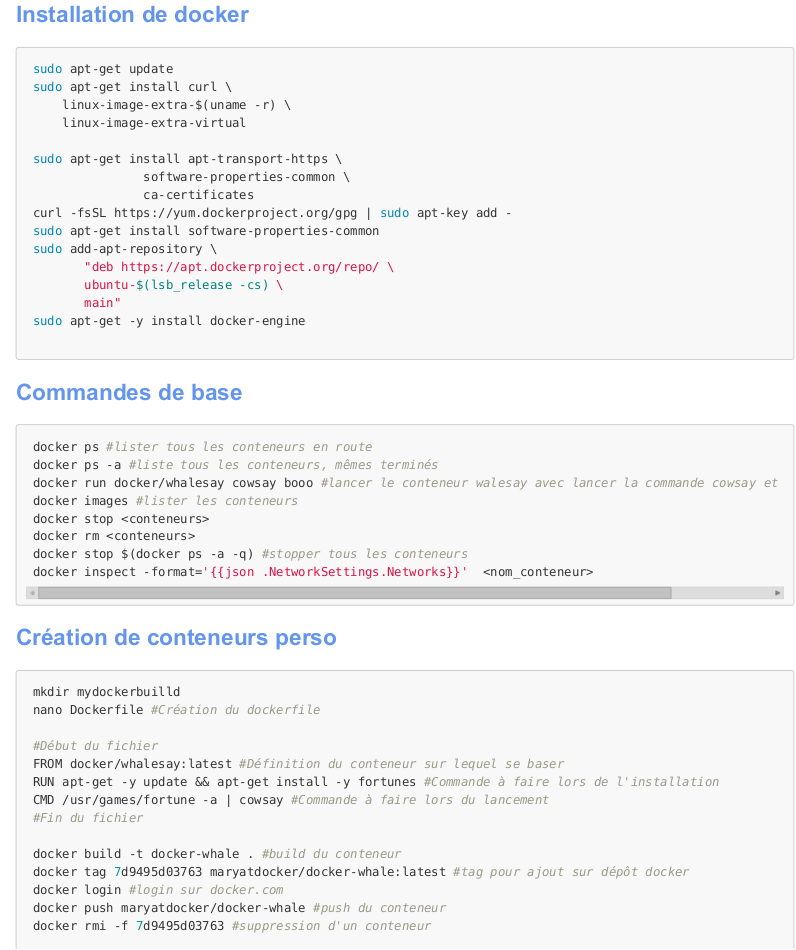
\includegraphics[scale=0.85]{docker1.png}
\newpage
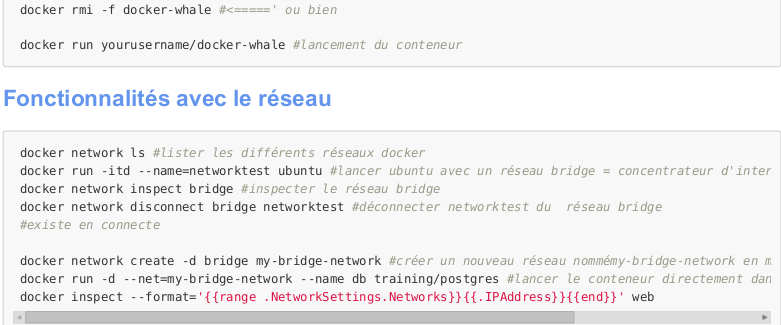
\includegraphics[scale=0.85]{docker22.png}
\section{LXC MEMO}
\subsection{Réseaux privé}
\subparagraph{Script UP }
Script pour up un réseaux prive dans LXC. 
\inputminted{bash}{script/LXC/private-up.sh}
\subparagraph{Script DOWN }
Script pour down un réseaux prive dans LXC .
\inputminted{bash}{script/LXC/private-down.sh}
\subparagraph{CONFIG }
Fichier de config du conteneur pour un  réseaux prive dans LXC. 
\inputminted{bash}{script/LXC/LXC_RP_CONF}

\subsection{Full bridge}
\subparagraph{Script UP }
\inputminted{bash}{script/LXC/fb-up.sh}
\subparagraph{Script DOWN }
\inputminted{bash}{script/LXC/fb-down.sh}
\subparagraph{CONFIG }
\inputminted{bash}{script/LXC/config_lxc_FB}

\subsection{OpenVSwitch}

\inputminted{bash}{script/LXC/command_b_openvSwitch}

\subsection{Bridge NAT}
\inputminted{bash}{script/LXC/config_lxc_BN}
\inputminted{bash}{script/LXC/bn-up.sh}
\inputminted{bash}{script/LXC/bn-down.sh}


\subsection{Ligne de commande utiles}
\inputminted{bash}{script/LXC/lxc_cl_usefull}
\section{KVM MEMO}
\inputminted{bash}{script/KVM/kvm_cl_utils}
\section{QEMU MEMO}
\inputminted{bash}{script/QEMU/gestDisk.txt}
\section{VitualBox MEMO}

\section{Config du /etc/network/interfaces de la Proxmox initial}
\inputminted{bash}{config.txt}


\newpage
\begin{thebibliography}{9}

 
  
      
\end{thebibliography}

\end{document}